\section{Árvores de ataque}
\label{sec:arvores}

O terceiro artefato (\texttt{docs/03-attack-trees.md}) desdobra cada caso de abuso numa árvore de ataque \parencite{schneier1999}. A árvore é o mapa do território, não o roteiro do jogo: lista os caminhos conhecidos para o objetivo do atacante. A raiz é o objetivo e as folhas são ataques concretos e executáveis; um conector OR significa que basta um caminho, e um AND, que todos os filhos são necessários. Cada folha vira um teste de regressão com o nome dela (por exemplo, T-F1.2) e tem um estado avaliado a cada build: \emph{aberta}, quando o ataque tem sucesso, ou \emph{fechada}, quando o controle resiste. A árvore não muda entre as builds; o que muda é a coluna de estados, que deve ficar mais fechada a cada iteração.

\subsection{Árvore 1: usar o aplicativo sem licença válida}

A Figura~\ref{fig:arvore1} reproduz o diagrama da árvore 1 que está no repositório, desenhado no início do projeto com o estado da build 0, e o Quadro~\ref{qd:arvore1} lista as folhas.

\begin{figure}[htbp]
\centering
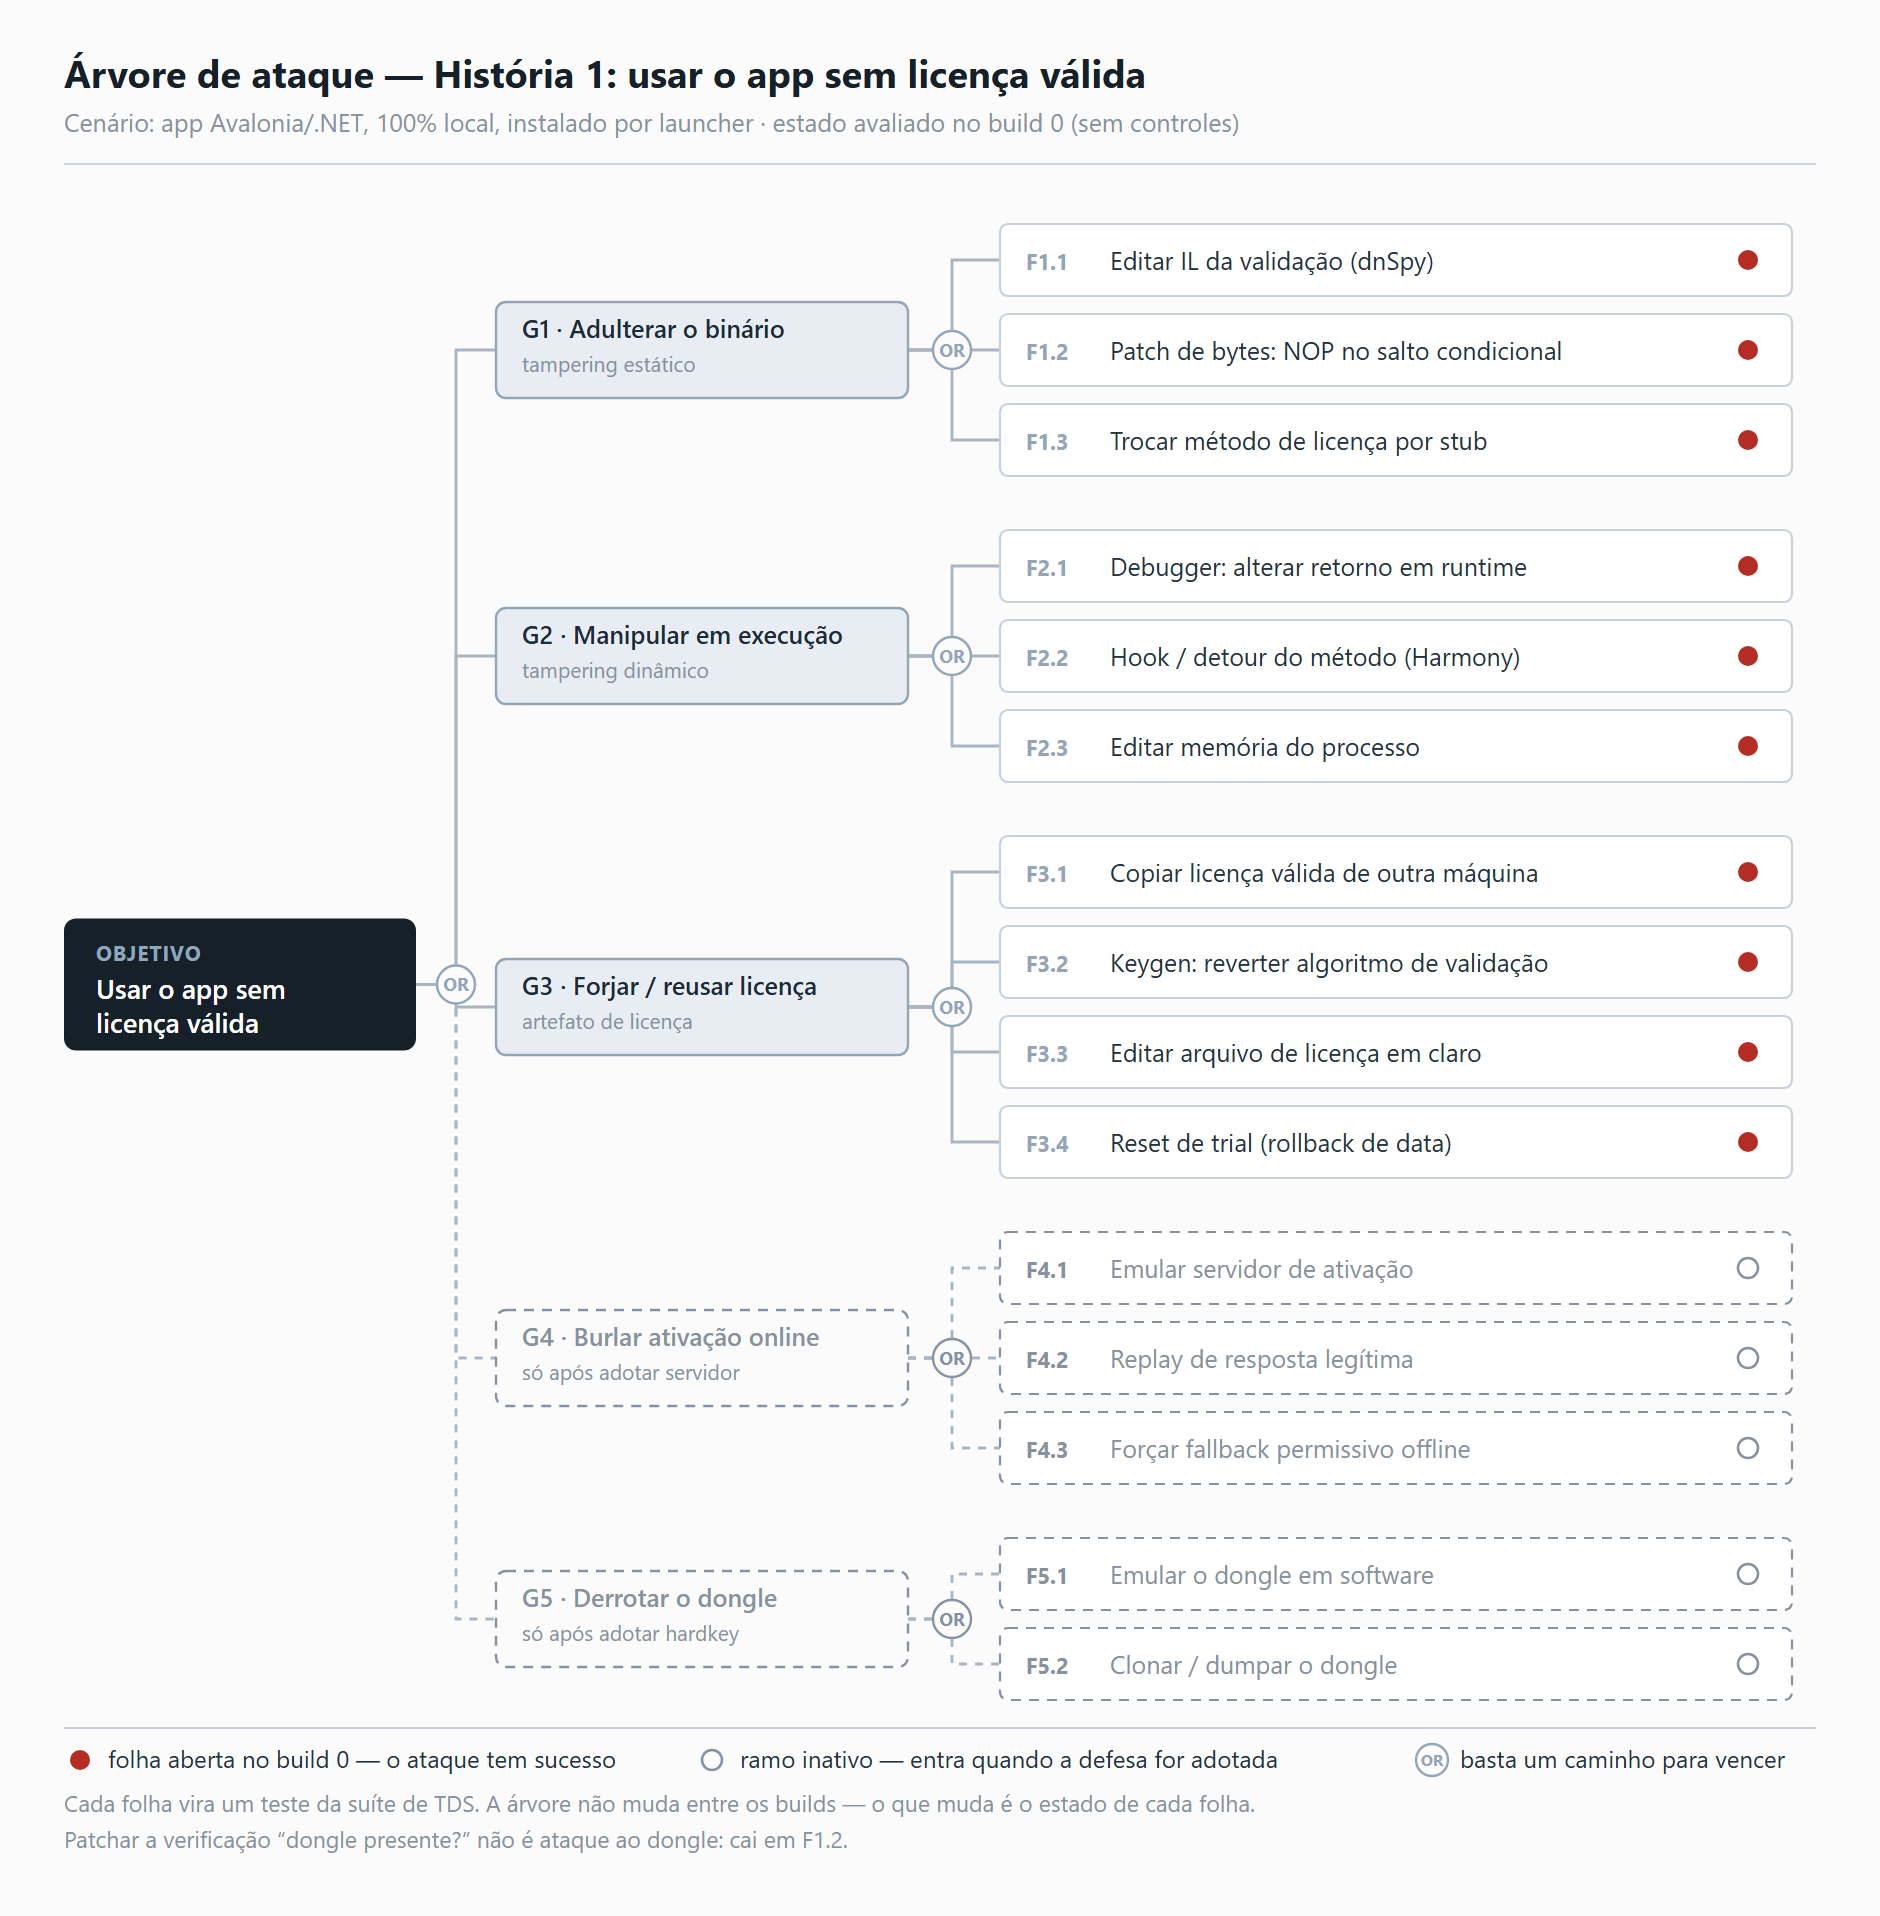
\includegraphics[width=0.92\textwidth]{arvore-ataque-1.png}
\caption{Árvore de ataque da história 1, no estado da build 0, como desenhada no início do projeto. Depois, a folha F3.4 ficou inativa, porque o mock não tem período de avaliação.}
\label{fig:arvore1}
\end{figure}

\begin{table}[htbp]
\centering
\caption{Folhas da árvore 1 (raiz OR).}
\label{qd:arvore1}
\small
\begin{tabular}{L{4.4cm}L{1.2cm}L{8.8cm}}
\toprule
Ramo & Folha & Ataque \\
\midrule
G1, adulterar o binário (tampering estático, OR) & F1.1 & Editar o IL da validação (dnSpy, ILSpy) e salvar o assembly \\
 & F1.2 & Patch de bytes: NOP no salto condicional \\
 & F1.3 & Substituir o método de licença por um stub que sempre libera \\
\midrule
G2, manipular em execução (tampering dinâmico, OR) & F2.1 & Depurador: alterar o retorno da validação em runtime \\
 & F2.2 & Hook ou detour do método (por exemplo, Harmony) \\
 & F2.3 & Editar a memória do processo (flag de licenciado) \\
\midrule
G3, forjar ou reusar a licença (OR) & F3.1 & Copiar uma licença válida de outra máquina \\
 & F3.2 & Keygen: reverter o algoritmo de validação \\
 & F3.3 & Editar o arquivo de licença em claro \\
 & F3.4 & Reset do período de avaliação (inativa: o mock não tem trial) \\
\midrule
G4, contornar ativação online (inativo) & F4.1 a F4.3 & Emular o servidor, replay de resposta legítima, forçar o modo offline permissivo \\
\midrule
G5, derrotar a hardkey (inativo) & F5.1 e F5.2 & Emular o dongle em software, clonar o conteúdo do dongle \\
\bottomrule
\end{tabular}
\end{table}

A árvore ensina duas coisas antes de qualquer ataque. Primeiro, enquanto o binário puder ser adulterado (G1 e G2), qualquer sofisticação em G3, G4 ou G5 é contornável por cima: patchear a verificação \enquote{a licença é válida?} não é atacar a licença, é cair em F1.2. A raiz real do problema é a integridade do binário. Segundo, G4 e G5 nascem inativos: só entram em jogo quando o blue team adotar aquele controle, mas os caminhos já estão desenhados de antemão.

\subsection{Árvore 2: recuperar o algoritmo proprietário}

\begin{table}[htbp]
\centering
\caption{Folhas da árvore 2 (raiz OR).}
\label{qd:arvore2}
\small
\begin{tabular}{L{4.4cm}L{1.2cm}L{8.8cm}}
\toprule
Ramo & Folha & Ataque \\
\midrule
H1, leitura direta (OR) & H1.1 & Descompilar o assembly e ler o algoritmo \\
 & H1.2 & Extrair parâmetros e pesos de configuração \\
\midrule
H2, compreender o algoritmo localizado (AND) & H2.1 & Localizar o módulo do algoritmo no binário \\
 & H2.2 & Compreender a lógica: nomes, fluxo e matemática \\
\bottomrule
\end{tabular}
\end{table}

O ramo H2 é um nó AND: para roubar de forma útil, o atacante precisa localizar e compreender. É exatamente onde a ofuscação atua, encarecendo H2.2. Na medição, o red vence a árvore 2 quando entrega uma reimplementação que reproduz a saída do stub num sinal de entrada que não viu, um oráculo. E, por ser AND, o custo de um caminho por H2 é a soma de localizar e compreender: localizar sozinho não rouba nada. A árvore também registra o teto honesto do MATE: nenhuma folha dela fecha em definitivo enquanto o algoritmo estiver no cliente.

Somando as duas árvores, são 13 folhas ativas (F1.1 a F1.3, F2.1 a F2.3, F3.1 a F3.3, H1.1, H1.2, H2.1 e H2.2) e três ramos ou folhas inativos até que o controle correspondente exista (F3.4, G4 e G5).
